\documentclass{article}
\usepackage[utf8]{inputenc}
% important for graphicx
\usepackage{graphicx}
\graphicspath{{img/}{src/}}
\usepackage{float}
\usepackage{hyperref}
\usepackage{enumitem}
\usepackage{algorithm}
\usepackage{subcaption}
\usepackage[mathscr]{euscript}
\usepackage[detect-all]{siunitx}
\usepackage[noend]{algpseudocode}
% background color for definitions
\usepackage[most]{tcolorbox}
\tcbset{
    frame code={}
    center title,
    left=0pt,
    right=0pt,
    top=0pt,
    bottom=0pt,
    colback=blue!6!white,
    colframe=white,
    width=\dimexpr\textwidth\relax,
    enlarge left by=0mm,
    boxsep=10pt,
    arc=0pt,outer arc=0pt,
}


\newenvironment{changemargin}[2]{%
\begin{list}{}{%
\setlength{\topsep}{0pt}%
\setlength{\leftmargin}{#1}%
\setlength{\rightmargin}{#2}%
\setlength{\listparindent}{\parindent}%
\setlength{\itemindent}{\parindent}%
\setlength{\parsep}{\parskip}%
}%
\item[]}{\end{list}}

\begin{document}

\title{Image Processing II\\
 Watershed}
\author{Aadil Anil Kumar \\
Otmane Sabir
}
\date{29/2/2020}
\maketitle
\vspace{10mm}
\begin{center}
\section*{Introduction}
\large
The second homework assignment required us to implement the watershed transform while following certain guidelines which could be summarized to the following list: 
\vspace{7mm}
\begin{enumerate}
    \item Implement the watershed algorithm as described as pseudo code from the \hyperref[sec:hello]{\textcolor{blue}{textbook}} 4-connected and 8-connected neighborhood.
    \item Output a single CSV file for the transformed image in the same format and same definition and value domains as the input image 'f'.
    \item Do meaningful (motivated from a real-world perspective) watersheds for 3 other images.
\end{enumerate}
\end{center}
\newpage

\tableofcontents

\newpage

\section{Watershed Transform}
\vspace{2mm}
\begin{flushleft}
The watershed transform is a classical segmentation - separating different objects in an image - algorithm in the world of image processing; it initially derives from the the geological watershed which means the elevated terrain that separates neighboring drainage basins. The watershed transform segmentation follows the same logic: starting from defined markers, the watershed algorithm treats pixels values as a local topography (elevation). The algorithm floods basins from the markers until basins attributed to different markers meet on watershed lines. \textit{See Figure \ref{fig:watershed_visualization}}\newline
\vspace{2mm}
\end{flushleft}
\begin{figure}[ht]
    \centering
    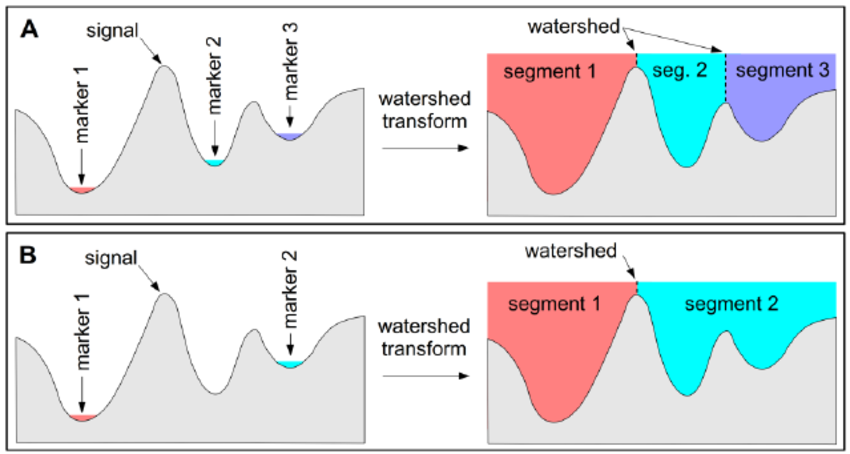
\includegraphics[width=8cm]{watershed.png}
    \caption{Watershed Visualization}
    \label{fig:watershed_visualization}
\end{figure}
\subsection{Formal Definition:}
\begin{flushleft}
\vspace{2mm }
\begin{tcolorbox}
\textsc{Definition:}\cite{parwshed}\newline\newline
Let $f \in C(D)$ have $minima$ $\{m_{k}\}_{k \in I}$, for some index set $I$. The catchment basin $CB(m_i)$ of a minimum $m_i$ is defined as the set of points $x \in D$ which are topographically closer to $m_i$ than to any other regional minimum $m_j$:
\begin{center}
\begin{equation*}
CB(m_i) = \{x \in D | \forall j \textbackslash \in I\{i\} : f(m_i) + T_f(x, m_i) < f(m_j) + T_f(x, m_j)\}
\end{equation*}
\end{center}
\vspace{2mm}
The watershed of $f$ is the set of points which do not belong to any catchment
\begin{center}
\begin{equation*}
Wshed(f) = D \cap \left(\bigcup\limits_{i \in I} CB(m_i)\right)^c.
\end{equation*}
\end{center}
\vspace{4mm}
Let $W$ be some label, $W \notin I$. The watershed transform of $f$ is a mapping $\lambda : D \to I \cup \{W\}$, such that $\lambda(p) = i$ if $p \in CB(m_i)$, and $\lambda(p) = W$ if $p \in Wshed(f)$.
\newline\newline\newline
So the watershed transform of $f$ assigns labels to the points of $D$, such that $(i)$ different catchment basins are uniquely labelled, and $(ii)$ a special label $W$ is assigned to all points of the watershed of $f$.
\end{tcolorbox}
\end{flushleft}
\section{Algorithmic Definition}
\vspace{2mm}In our implementation, we're relying on the simulated immersion approach introduced by Vincent \& Soille\cite{soilletextbook}.\newline\newline
Metaphorically speaking, the algorithm pierces holes in every minimum, and the entire relief begins to be flooded with water. Starting from the minimum of lowest height, the water gradually fills up all catchment basins. Watersheds are built in the places where water from different basins unites. The process ends when the water reaches the maximum peak of the relief, and as a result, every catchment basin gets covered by the watershed lines which are easily distinguishable lines from the rest of the output.
\subsection{Formal Definition}
\begin{tcolorbox}
\textsc{Definition 2:}\cite{parwshed}\newline\newline
Let $f : D \to \N$ be a digital grey value image, with $h_{min}$ and $h_{max}$ the minimum and maximum value of $f$. Define a recursion with the grey level $h$ increasing from $h_{min}$ to $h_{max}$, in which the basins associated with the minima of f are successively expanded. Let $X_h$ denote the union of the set of basins computed at level $h$. A connected component to the threshold set $T_{h + 1}$ at level $h + 1$ can be either a new minimum, or an extension of a basin in $X_h$: in the latter case one computes the geodesic influence zone of $X_h$ within $T_{h+1}$, resulting in an update $X_{h+1}$. Let $MIN_h$ denote the union of all regional minima at altitude h.\newline\newline
Let us now define the following recursion: \newline
\[
\begin{cases}
    X_{h_{min}} = & \{p \in D | f(p) = T_{h_{min}}\}\\
    X_{h+1} = & MIN_{h+1} \cup IZ_{T_{h+1}}\left(X_h\right), h \in [h_{min}, h_{max})
\end{cases}
\]
\newline\newline
The watershed $Wshed(f)$ of $f$ is the complement of $X_{h_{max}}$ in $D$ : 
\begin{center}
    $Wshed(f) = D \textbackslash X_{h{max}}$
\end{center}
\end{tcolorbox}
\vspace{2mm}
\begin{flushleft}
Let's use Figure \ref{fig:example_1} from \cite{parwshed} as an example of the algorithm defined above. Assuming that A and B are basin labels and that W is the watershed pixels. Then the algorithm will proceed as shown in the figure (a) is the original image and the (b-e) are steps following the algorithm definition above.
\end{flushleft}

\begin{figure}[H]
    \centering
    \includegraphics[width=\linewidth]{example1.png}
    \caption{Immersion algorithm on the 4-connected grid}
    \label{fig:example_1}
\end{figure}

\subsection{Implementation}
As we previously discussed, we attempted to implement the immersion approach. The pseudo code \href{alg:immersion_alg} below was provided by Soille \cite{soilletextbook}.
\newline
\subsubsection{Pixel Mapping}
\label{sec:pixel_mapping}
\begin{flushleft}
One of the main challenges we encountered during the implementation of the algorithm was mapping the pixels using their indices to their specific locations and gray values. First, we tried getting all the pixels using the image itself but then found a better solution which doesn't require any information from the image besides its height and width - we'll refer to these values as \textit{H} \& \textit{W} respectively. The idea is to generate a matrix of the same H and W and assign it x, y values the same way they would be assigned to a grid. The idea is creating two matrices, one where we create a row ranging from \numrange[range-phrase = --]{0}{W} and duplicate it over H number if times. We then create a second matrix where rows are a constant value \textit{C} repeated width times and the columns increment \textit{C} by one after each iteration ranging from \numrange[range-phrase = --]{0}{H}. We then take these matrices, reshaped them in the format of a list of 2 element arrays and transpose it to get our [y, x] mapping.
\end{flushleft}
\subsubsection{Neighbouring Pixels}
\begin{flushleft}
The neighbouring pixels follows the same logic as the previous section but with a different way of interpreting the range.  We decided to use a combination of the pixel mapping logic but also by introducing a different way to limit how far we go. We first get the maximum and minimum values of the given pixel. This allows us to first find whether the current pixel is at a border and also allows to avoid having an issue with a negative value. As all of our output is initialized with a -1 value. We then generate two matrices in a similar fashion to the previous section \ref{sec:pixel_mapping} and perform similar matrix handling operations in order to obtain a mapping of these pixels. We also allowed the user to freely pick a number of pixels which we divide by 2 in order to make sure we're not giving more than what the user is asking for. This also made it easier for us to experiment with differently sized number of neighbors in our future sections.
\end{flushleft}

\newpage

\vspace*{-3cm}

\begin{algorithm}[H]
\caption{Watershed using flooding simulations}\label{euclid}
\begin{algorithmic}[1]
\label{alg:immersion_alg}
\Procedure{watershed}{}
\State $\textit{mask} \gets \text{-2  ;  }  \textit{initial value of a threshold level}$
\State $\textit{wshed} \gets \text{0  ;  }  \textit{value of pixels belonging to watersheds}$
\State $\textit{inqueue} \gets \text{-3  ;  } \textit{value assigned to pixels put into the queue}$
\State $\textit{init} \gets \text{-1  ;  } \textit{initial value of f0)}$
\newline
\State \emph{Input : $f_i$}, \text{grey tone image (non negative integers)}:
\State \emph{Output : $f_0$}, \text{image of labelled catchment basins}:
\newline
\Procedure{Initialisations}{}
\State \text{Value} \emph{$f_i$} \text{is assigned to each pixel of $f_0$}:
\State \emph{current\_label} $\gets$ \text{0}:
\State \emph{flag: } \text{Boolean variable}:
\State \emph{$N(p)$} \text{is the set of neighbours of P}:
\EndProcedure
\newline
\State \textbf{Sort} the pixels of $f_i$ in the increasing order of their grey values. \newline
\For{$h \gets h_{min}$ \textbf{to} $h_{max}$}
\Comment{geodesic SKIZ of level h - 1 inside level h}
    \For{pixel p}
    \Comment{such that $f_{i}(p) = h$}
        \State $f_{0}(p) \gets$ \text{mask}
        \If{ $\exists$ p' $\in$ N(p) | $f_{0}(p') > 0$ \textbf{OR} $f_{0}(p')$ = wshed}
            \State \emph{$f_{0}(p) \gets$ inqueue}
            \Comment{fifo.add(p)};
        \EndIf
    \EndFor
\EndFor
\While{fifo.empty() = false}
    \State p $\gets$ fifo.retrieve();
    \For{pixel p' $\in N(p)$}
        \If{$f_{0}(p') > 0$}
        \Comment{i.e., p' belongs to an already labelled basin}
            \If{$f_{0}(p) = $ inqueue \textbf{OR} ($f_{0}(p) = $ wshed \textbf{\&} flag = true)}
                \State $f_{0}(p) \gets f_{0}(p')$
            \ElsIf{$f_{0}(p) >$  0 \textbf{AND} $f_{0}(p) \neq f_{0}(p')$}
                \State $f_{0}(p) \gets wshed$
                \Comment{flag $\gets$ false}
            \EndIf
        \EndIf
        \ElsIf{$f_{0}(p') =$ wshed}
            \If{$f_{0}(p) = $inqueue}
                \State $f_{0}(p) \gets$ wshed;
                \State flag $\gets$ true;
            \EndIf
        \ElsIf{$f_{0}(p')$ = ,ask}
            \State $f_{0}(p) \gets$ inqueue;
            \State $f_{0}(p') \gets$ mask;
        \EndIf
    \EndFor
    \For{pixel p} 
    \Comment{such that $f_{i}(p)$ = mask}
        \If{$f_{0}(p)$ = mask}
        \Comment{check for new minima}
            \State current\_label $\gets$ current\_label + 1;
            \State fifo.add(p);
            \State $f_{0}(p) \gets $ current\_label;
            \While{fifo.empty() = false}
                \State $p' \gets$ fifo.retrieve();
                \For{p" $\in N(p')$}
                    \If{$f_{0}(p'')$ = mask}
                        \State fifo.add(p'');
                        \State $f_{0}(p'') \gets$ current\_label;
                    \EndIf
                \EndFor
            \EndWhile
        \EndIf
    \EndFor    
\EndWhile
\EndProcedure
\end{algorithmic}
\end{algorithm}

\begin{figure}[H]
    \centering
    \includegraphics[width=\linewidth]{neighbor-chartbar.png}
    \caption{Different neighbors bar chart.}
    \label{fig:neighbor-chartbar}
\end{figure}

\section{Experiments \& Results}
Please find all the experimental outputs in the outputs folder of the directory.
\subsection{Test Input 1}
f1\_dinv is a signed image blob. We compute the distance transformation of f1 to derive the appropriate graylevel intensities of pixels inside the foreground region to show the distance to the closest boundary from each pixel.
\begin{figure}[ht]
\centering
\begin{subfigure}{.5\textwidth}
  \centering
  
\includegraphics[scale=10]{experiments/f1_f2/f1_distanced.png}
  \caption{Distance transformation of f1}
  \label{fig:f1_1}
\end{subfigure}%
\begin{subfigure}{.5\textwidth}
  \centering
  \includegraphics[scale=10]{experiments/f1_f2/4_f1_segmented.png}
  \caption{Watershed with 4 Neighbours of f1}
  \label{fig:f1_2}
\end{subfigure}
\caption{Results of experiments on f1}
\label{fig:f1}
\end{figure}
\begin{flushleft}
Figure \ref{fig:f1_2} show us the result of applying the watershed algorithm to Figure \ref{fig:f1_1}, we arrive at an image that depicts a 8-bit sword. 
\end{flushleft}

\subsection{Test Input 2}
f2 is also a signed blob. By saving it as an image, figure \ref{fig:f1} shows us that f2 is an image containing different circles.
\begin{figure}[ht]
    \centering
    \includegraphics[scale=.5]{experiments/f1_f2/f2.png}
    \caption{f2 as jpg}
    \label{fig:f2}
\end{figure}

\begin{flushleft}
We proceed to apply the watershed algorithm to the image. 
\end{flushleft}
\begin{figure}[ht]
\centering
\begin{subfigure}{.5\textwidth}
  \centering
  \includegraphics[scale=.6]{experiments/f1_f2/4_f2_segmented.jpg}
  \caption{Watershed with 4 Neighbours of f2}
  \label{fig:f2_1}
\end{subfigure}%
\begin{subfigure}{.5\textwidth}
  \centering
  \includegraphics[scale=.6]{experiments/f1_f2/8_f2_segmented.jpg}
  \caption{Watershed with 8 Neighbours of f2}
  \label{fig:f2_2}
\end{subfigure}
\caption{Results of experiments on f2}
\label{fig:f2_ex}
\end{figure}
\subsubsection{Interpretation}
\begin{flushleft}
Figure \ref{fig:f2_1} shows us that using 4 neighbours for water-shedding results in a over-segmented image. On the other hand, figure \ref{fig:f2_2} shows us that using 8 neighbours for water-shedding results in an image having fewer regions.
In general, the more neighbours that you have the lower the amount of regions that are present in the resulting image. This occurs due to the algorithm simultaneously creating larger regions beginning at the initial regional minima. For each regional minimum, each iteration of the 8-connected algorithm uses a bigger region to classify the minimum's neighbours, resulting in larger but fewer regions. 

\end{flushleft}

\subsection{Nuclei Segmentation}
\begin{flushleft}
One of the many uses of segmentation is with nuclei. Cell nuclei are important indicators of cellular process and diseases and power of image processing has been able to automate this process in order to gain further insight into cells, their features, and functionalities. Therefore
, we decided to also test the efficiency of our immersion watershed in splitting heavily clustered nuclei.
\end{flushleft}

\subsubsection{Results}
\begin{flushleft}
The results we obtained were after heavy processing and show how the combination of different filters and algorithms can help us obtain the needed results.
\end{flushleft}
\begin{figure}[H]
    \centering
    \includegraphics[width=.6\linewidth]{experiments/nuclei/nuclei.png}
    \caption{Original Cell Nuclei Image.}
    \label{fig:cell_nuclei}
\end{figure}
\begin{flushleft}
We first started by directly applying the watershed transform to this image without any sort of prepossessing or filters, see Figure \ref{fig:nuclei_main}. One of the first things we noticed is how the segmentation works inversely. As it's trying to remove the nuclei but maintain the background; therefore, the first step was to apply an inverse (bit-wise not) filter in order to invert the image - this allows us to shift focus on the nuclei. We also noticed how the image noise and nuclei cell clusters are causing the image to over segment regardless which made us think of different filters which will reduce this noise and also maintain the edges to a certain extent and the best fit was the blur filter.
\end{flushleft}
\begin{figure}[H]
\centering
\begin{subfigure}{6cm}
  \centering
  \includegraphics[width=6cm]{experiments/nuclei/4_nucleiseg.png}
  \caption{4 Neighbors}
\end{subfigure}    
\begin{subfigure}{6cm}
  \centering
  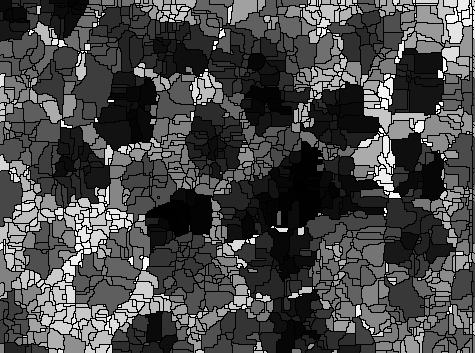
\includegraphics[width=6cm]{experiments/nuclei/8_nucleiseg.png}
  \caption{8 Neighbors}
\end{subfigure}
\caption{Applying watershed only}
\label{fig:nuclei_main}
\end{figure}
\begin{flushleft}
After applying both the blur \& the inverse, see Figure \ref{fig:nuclei_bluronly}. These results showed less segmentation and undesired effects but allowed us to come up with two conclusions. First, that the 4-neighbor watershed is not very helpful and its results are not valid; therefore, we decided to mainly rely on the 8-neighbors watershed as it was showing more prominent results. Second, the average blur filter was very helpful in getting rid of over-segmentation but we now wanted to compare its results to a different filter the bilateral filter.
\end{flushleft}
\begin{figure}[H]
\centering
\begin{subfigure}{6cm}
  \centering
  \includegraphics[width=6cm]{experiments/nuclei/4Blur_nucleiseg.png}
  \caption{4 Neighbors}
\end{subfigure}    
\begin{subfigure}{6cm}
  \centering
  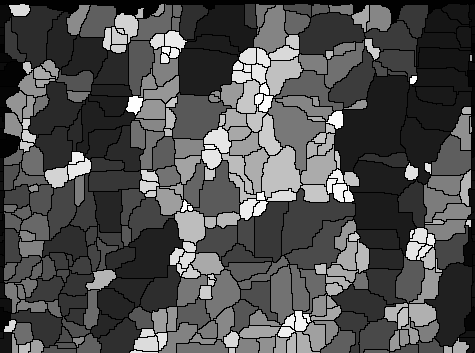
\includegraphics[width=6cm]{experiments/nuclei/8Blur_nucleiseg.png}
  \caption{8 Neighbors}
\end{subfigure}
\caption{Watershed with a median blur filter.}
\label{fig:nuclei_bluronly}
\end{figure}
\begin{flushleft}
After applying both filters, see Figure \ref{fig:nuclei_blurcomp}, we noticed that while the bilateral filter does define basins better it also over segments the image a little more than the median filter and since these results were not conclusive enough for us to pick one of these filters we decided to carry our tests with both of them until one proves to give better results the other. Since the segmentation was still not producing the results we were expecting, we decided to add more processing and adaptive threshold was the next step.
\end{flushleft}
\begin{figure}[H]
\centering
\begin{subfigure}{6cm}
  \centering
  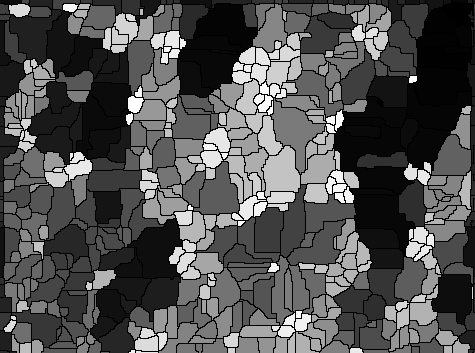
\includegraphics[width=6cm]{experiments/nuclei/bilateral_nucleiseg.png}
  \caption{Bilateral Blur Filter.}
\end{subfigure}    
\begin{subfigure}{6cm}
  \centering
  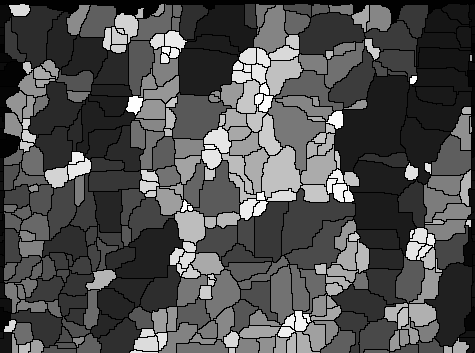
\includegraphics[width=6cm]{experiments/nuclei/median_nucleiseg.png}
  \caption{Median Blur Filter.}
\end{subfigure}
\caption{8-neighbor watershed using different blur filters.}
\label{fig:nuclei_blurcomp}
\end{figure}
\begin{flushleft}
The adaptive threshold was maybe one of the most important steps towards getting better results. The algorithm determines the threshold for a pixel based on a small region around it. So we get different thresholds for different regions of the same image which gives better results for images with varying illumination. The results were a big improvement and this also where we started noticing big differences between the median and bilateral filters. As we can see in figure \ref{fig:nuclei_thresh}
\end{flushleft}
\begin{figure}[H]
\centering
\begin{subfigure}{6cm}
  \centering
  \includegraphics[width=6cm]{experiments/nuclei/bilateralThresh_nucleiseg.png}
  \caption{Bilateral Blur.}
\end{subfigure}    
\begin{subfigure}{6cm}
  \centering
  \includegraphics[width=6cm]{experiments/nuclei/medianThres_nucleiseg.png}
  \caption{Median Blur.}
\end{subfigure}
\caption{8-neighbor watershed with adaptive threshold.}
\label{fig:nuclei_blurcomp}
\end{figure}
\begin{flushleft}
We now decided to give it one more change and increase the image contrast. That would allow us to completely dim out the dark areas and make the other ones more visible. Surprisingly, this gave better results in general, see Figure \ref{fig:nuclei_threshFinal} and we were now finally able to completely view these segmented cells. The nuclei is now marked in a different color and a lot of the information that we don't need is filtered out. This left us with a lot better results generally and also concluded that a median blur is what we need in this case.
\end{flushleft}
\begin{figure}[H]
\centering
\begin{subfigure}{6cm}
  \centering
  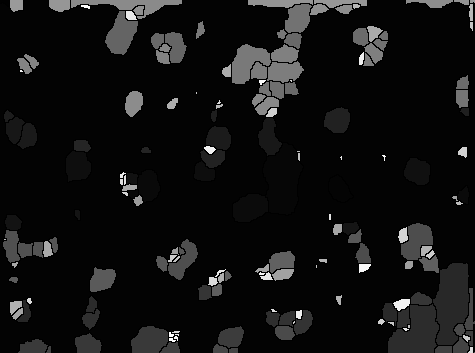
\includegraphics[width=6cm]{experiments/nuclei/finalBilateral_nucleiseg.png}
  \caption{Bilateral Blur.}
\end{subfigure}    
\begin{subfigure}{6cm}
  \centering
  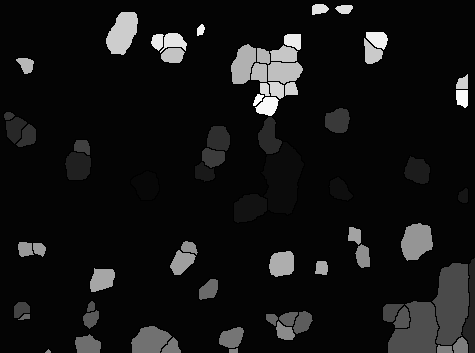
\includegraphics[width=6cm]{experiments/nuclei/finalMedian_nucleiseg.png}
  \caption{Median Blur.}
\end{subfigure}
\caption{8-neighbor Watershed with all filters.}
\label{fig:nuclei_threshFinal}
\end{figure}

\subsubsection{Conclusion}
\begin{flushleft}
This serves as a good example, see Figure \ref{fig:nuclei_final} to show how much pre-processing an image can give much better results. 
\end{flushleft}
\begin{figure}[H]
\centering
\begin{subfigure}{6cm}
  \centering
  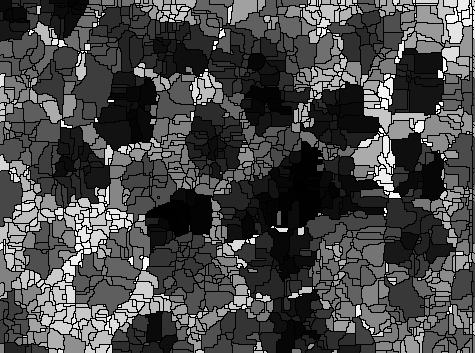
\includegraphics[width=6cm]{experiments/nuclei/8_nucleiseg.png}
  \caption{Initial 8-Neighbour Segmentation.}
\end{subfigure}    
\begin{subfigure}{6cm}
  \centering
  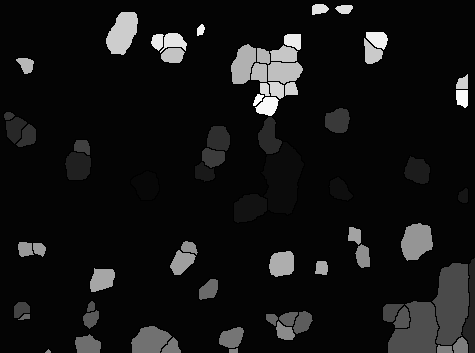
\includegraphics[width=6cm]{experiments/nuclei/finalMedian_nucleiseg.png}
  \caption{Final result.}
\end{subfigure}
\caption{8-neighbor Nuclei Watershed.}
\label{fig:nuclei_final}
\end{figure}



% ---------------------I END HERE-----------------
\subsection{Brain MRI Slice Segmentation}

\begin{flushleft}
Another valid use of segmentation functions in the realm of medical image processing is segmenting MRI slices of the brain. This is done in order to isolate different structures and tissues within the brain to check for the existence of any abnormalities pertaining to an individuals medical condition. These abnormalities could be identified by tracking changes in volume, shape and regional distribution of brain tissue during by comparing it to previous scans. 
\end{flushleft}

\subsubsection{Results and Interpretations}
\begin{figure}[H] % just forcing its position OK
    \centering
    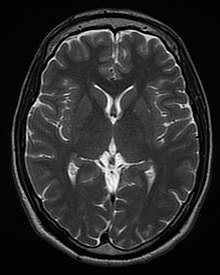
\includegraphics[scale=.6]{experiments/brain/brain.jpg}
    \caption{Original image of the brain.}
    \label{fig:brain_1}
\end{figure}
\begin{flushleft}
The MRI Slice is a gray scale image. We begin by first directly applying the watershed transform to the image without the use of any morphological pre-processing, figure \ref{fig:brain} depicts these results.
\end{flushleft}
\begin{figure}[H] %same here
\centering
\begin{subfigure}{.5\textwidth}
  \centering
  \includegraphics[scale=0.6]{experiments/brain/4_brain_segmented.jpg}
  \caption{Watershed (4-Neighbours) of image.}
  \label{fig:brain_2}
\end{subfigure}%
\begin{subfigure}{.5\textwidth}
  \centering
  \includegraphics[scale=0.6]{experiments/brain/8_brain_segmented.jpg}
  \caption{Watershed (8-Neighbours) of image.}
  \label{fig:brain_3}
\end{subfigure}
\caption{Direct application of watershed to the image.}
\label{fig:brain}
\end{figure}

\begin{flushleft}
The original image, figure \ref{fig:brain_1}, shows the presence of some noise. Therefore, we proceed with applying a filter before segmenting the image. In terms of filter choice, since the brain contains a lot of peaks and troughs within it, we thought that it would be best to use a edge-preserving filter. The two options that we conducted experiments with were the median and bilateral filters, figure \ref{fig:brain2} depicts the results. 
\end{flushleft}
\begin{figure}[H]
\centering
\begin{subfigure}{.5\textwidth}
  \centering
  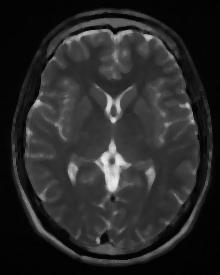
\includegraphics[scale=0.6]{experiments/brain/brainMed.jpg}
  \caption{Median filter}
  \label{fig:brain_4}
\end{subfigure}%
\begin{subfigure}{.5\textwidth}
  \centering
  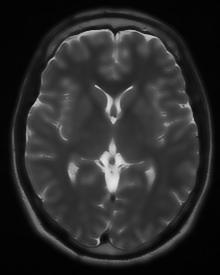
\includegraphics[scale=0.6]{experiments/brain/brainBil.jpg}
  \caption{Bilateral filter}
  \label{fig:brain_5}
\end{subfigure}
\caption{Application of filters to the original image.}
\label{fig:brain2}
\end{figure}
\begin{flushleft}
Figure \ref{fig:brain2} shows us that both filters result in an edge-preserved image. However, the bilateral filter results in a less noisy image, therefore, we shall now segment this image.
\end{flushleft}

\begin{flushleft}
Figure \ref{fig:brain3} shows us the results of segmenting the bilaterally filtered image. When comparing these results to figure \ref{fig:brain} we can see that we obtain a much better segmentation of the brain. This would allow for better time interval based comparisons of a person's brain scans.\newline\newline
Additionally, figure \ref{fig:brain_8} shows us the result of using 12 neighbours for the segmentation. Our implementation of the algorithm allows us to pick the amount of neighbours we want for each run. Although we are not exactly sure of how it works for neighbours $>$ 8, we assume that algorithm gets arbitrary neighbours of the neighbours of the current pixel being referenced.
\end{flushleft}

\begin{figure}[H]
\centering
\begin{subfigure}{6cm}
  \centering
  \includegraphics[scale=0.6]{experiments/brain/brainBL_4.jpg}
  \caption{4-Neighbours}
  \label{fig:brain_6}
\end{subfigure}    
\begin{subfigure}{6cm}
  \centering
  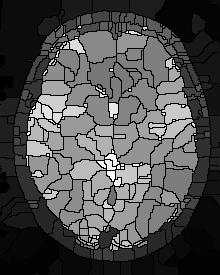
\includegraphics[scale=0.6]{experiments/brain/brainBL_8.jpg}
  \caption{8-Neighbours}
  \label{fig:brain_7}
\end{subfigure}
% \begin{subfigure}{6cm}
%   \centering
%   \includegraphics[width=5cm]{expescale=0.6riments/brain/brainM_16.jpg}
%   \caption{Inversion \& Median Blur \& Contrast}
%   \label{fig:nuclei_invMedConstrast}
% \end{subfigure}
\label{fig:brain3}
\caption{Applying watershed to the filtered image.}
\end{figure}
\begin{figure}[H]
  \centering
  \includegraphics[scale=0.6]{experiments/brain/brainBL_12.jpg}
  \caption{12-Neighbours}
  \label{fig:brain_8}
\end{figure}

% ---------------------I END HERE-----------------

\subsection{Animal Segmentation for Classification}
\begin{flushleft}
Image segmentation plays a key role in machine learning, particularly in image classification applications. In this experiment we try to segment a zebra (Larry) from its background of the Savannah. A segmented Larry could help deep learning algorithms classify him as a zebra.
\end{flushleft}

\subsubsection{Results and Interpretations}
\begin{figure}[H]
  \centering
    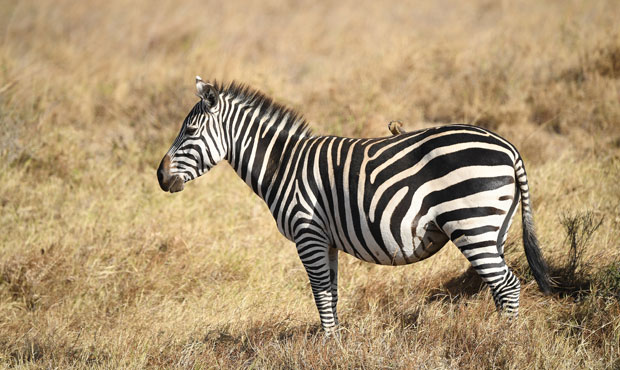
\includegraphics[scale=0.3]{experiments/zebra/zebra.jpg}
    \caption{Original image of a zebra}
    \label{fig:zebra_1}
\end{figure}
\begin{figure}[H]
  \centering
  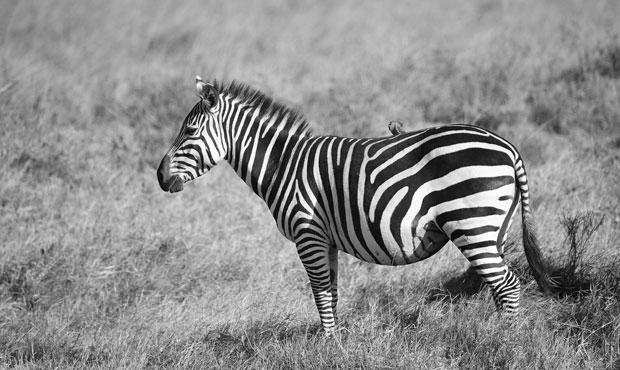
\includegraphics[scale=.3]{experiments/zebra/zebraGray.jpg}
  \caption{Gray scale image}
  \label{fig:zebra_2}
\end{figure}
\begin{flushleft}
We first convert the image to gray scale. Then we try to directly apply the watershed transform.
\end{flushleft}

\begin{figure}[H]
\centering
\begin{subfigure}{10cm}
  \centering
  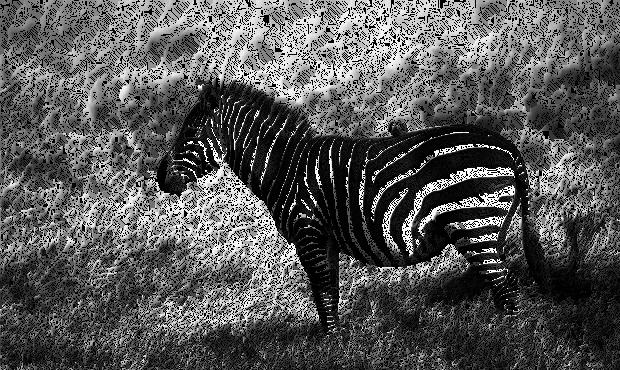
\includegraphics[scale=0.3]{experiments/zebra/4_zebra_segmented.jpg}
  \caption{4-Neighbours}
  \label{fig:zebra_3}
\end{subfigure}    
\begin{subfigure}{10cm}
  \centering
  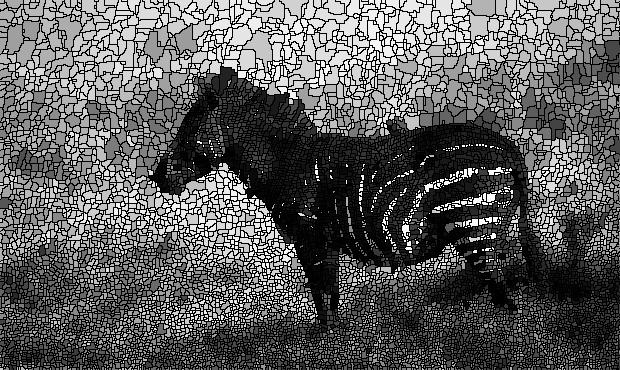
\includegraphics[scale=0.3]{experiments/zebra/8_zebra_segmented.jpg}
  \caption{8-Neighbours}
  \label{fig:zebra_4}
\end{subfigure}
\label{fig:zebra1}
\caption{Directly applying watershed to the image.}
\end{figure}
\begin{flushleft}
Once again, Figure \ref{fig:zebra1} shows us that the direct application of the watershed transform results in a heavily over-segmented image. In order to combat the over-segmentation we once again make use of the bilateral filter to preserve the edges while reducing the noise.
\end{flushleft}

\begin{flushleft}
Figure \ref{fig:zebra2} shows us that performing the segmentation after applying the filter results in fewer regions being formed in comparison to Figure \ref{fig:zebra1}. The foreground object (zebra) is much clearer in comparison to the background. This would ideally allow for segmenting the animal from its environment for classification. \newline \newline
However, the drawback of the immersion based watershed algorithm is evident by the persisting presence of many regions.  
\end{flushleft}

\begin{figure}[H]
\centering
\begin{subfigure}{10cm}
  \centering
  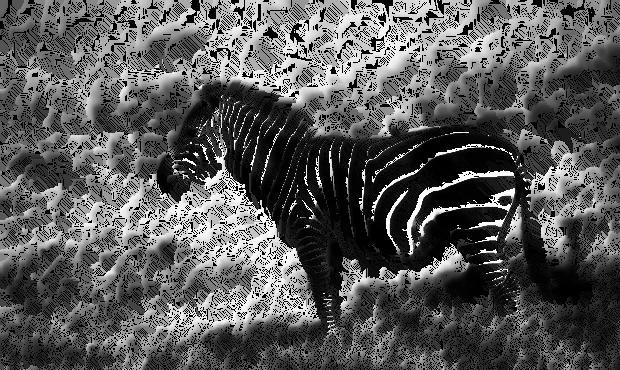
\includegraphics[scale=0.4]{experiments/zebra/zebraBL_4.jpg}
  \caption{4-Neighbours}
  \label{fig:zebra_5}
\end{subfigure}    
\begin{subfigure}{9cm}
  \centering
  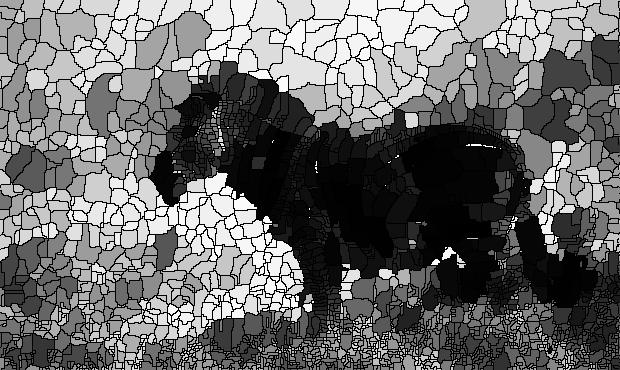
\includegraphics[scale=0.4]{experiments/zebra/zebraBL_8.jpg}
  \caption{8-Neighbours}
  \label{fig:zebra_6}
\end{subfigure}
\label{fig:zebra2}
\caption{Directly applying watershed to the image.}
\end{figure}

% ---------------------I END HERE-----------------
\section{Comparison}
The breadth-first implementation that we're discussing uses a FIFO (First in First Out) queue to find the level of pixels of constant grey value as we have seen, c.f Algorithm \ref{alg:immersion_alg}. For each of these thresholds a pixel is stored in the empty queue, followed by the 'flooding' which runs until the queue is empty. 
\subsection{Time Complexity}

\begin{flushleft}
We ran some tests on the algorithm which was presented in order to visualize the time complexity of this algorithm. 
We can clearly see that the time complexity is linear in the number of pixels in the image; however, 
the theoretical time complexity would change from linear to quadratic due to the repeated processing of the watershed pixel \cite{timecomplexity}.
\end{flushleft}
\begin{figure}[H]
\centering
\begin{subfigure}{.5\textwidth}
  \centering
  \includegraphics[width=\linewidth]{tests/performane_8.png}
  \caption{8 - Neighbours}
  \label{fig:sub1}
\end{subfigure}%
\begin{subfigure}{.5\textwidth}
  \centering
  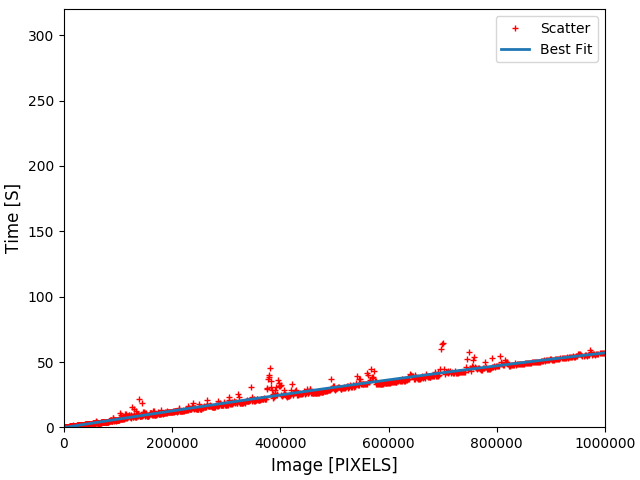
\includegraphics[width=\linewidth]{tests/performance_4.png}
  \caption{4 Neighbours}
  \label{fig:sub2}
\end{subfigure}
\caption{Scatter Plot  \& Best Fit curve of results}
\label{fig:general_test}
\end{figure}

\subsection{N-Neighbors Influence}
\begin{flushleft}
After the previous tests, we noticed how the number of neighbors scanned impacts the time the algorithm; therefore, we decided to run different test with various neighbor sizes (2, 4, 8, 16) and visualized the differences as seen in  Figure~\ref{fig:neighbor-test}. We ran a test on random graphs of size [n , n] with n ranging from \numrange[range-phrase = --]{1}{500}. We also ran a test, c.f \ref{fig:neighbor-chartbar} using 2, 4, 6, 8, 16, 32, and 64 to be able to determine how exactly the amount of neighbors influences the overall run time of the algorithm on a 512*512 image.

This helps us explain how the algorithm heavily depends on its neighbors and why, as previously mentioned, the time complexity can vary from linear to quadratic. We almost always see a doubling the overall time until we reach 64 neighbors and notice a much more significant jump.
\end{flushleft}

\begin{figure}[H]
    \centering
    \includegraphics[width=.7\linewidth]{neighbor-chartbar.png}
    \caption{Different neighbors bar chart.}
    \label{fig:neighbor-chartbar}
\end{figure}

\begin{figure}[H]
  \begin{subfigure}{6cm}
    \centering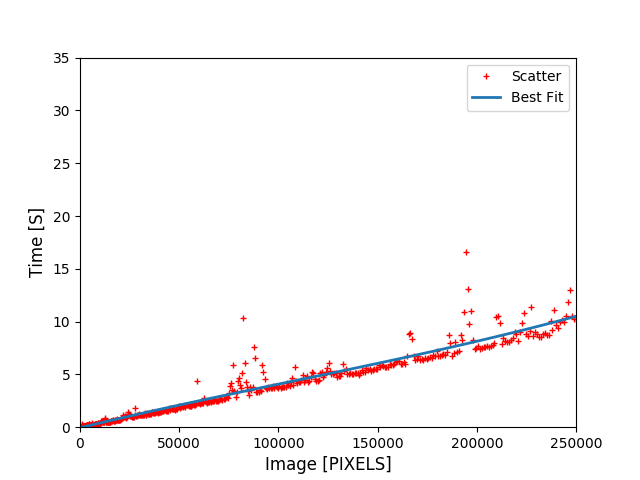
\includegraphics[width=6cm]{tests/test_ws_2.png}
    \caption{2 - Neighbors}
  \end{subfigure}
  \begin{subfigure}{6cm}
    \centering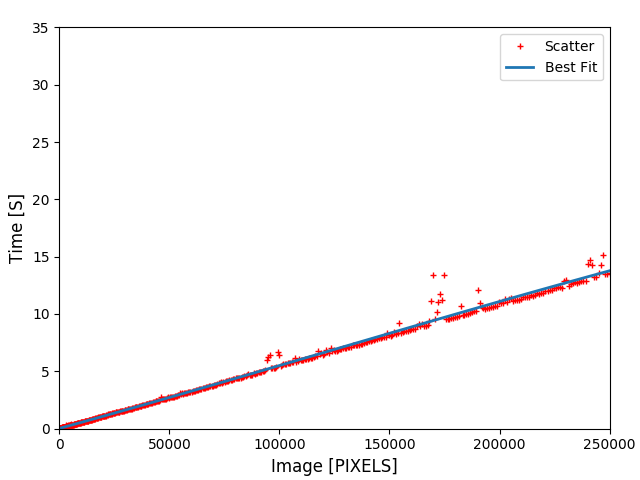
\includegraphics[width=5.5cm]{tests/test_ws_4.png}
    \caption{4 - Neighbors}
  \end{subfigure}
 
  \begin{subfigure}{6cm}
    \centering\includegraphics[width=6cm]{tests/test_ws_8.png}
    \caption{8 - Neighbors}
  \end{subfigure}
  \begin{subfigure}{6cm}
    \centering\includegraphics[width=5.5cm]{tests/test_ws_16.png}
    \caption{16 - Neighbors}
  \end{subfigure}
  \caption{Scatter Plot \& Best Fit curve for different neighbors}
  \label{fig:neighbor-test}
\end{figure}



\subsection{Disadvantages of the Queue}
\begin{flushleft}
One of the main advantages of this algorithm is how it utilizes the queue to reduce time complexity and keeps all our operations feasible in linear time but this also comes at a cost. When running our initial test, we tried running multiple processes at the same time in for optimal performance; however, we ran into many issues because of the nature of the algorithm. The required size of the queue is not known in advance, and memory is addressed in a very unstructured and "blind" manner, causing performance degradation on
virtual memory and especially on parallel computing, since it requires a lot of synchronization and tends to leave with many imprecise results. In the figures below you can clearly see the difference when running the processes concurrently vs. running them in normal linear manner.
\end{flushleft}

\begin{figure}[ht]
\centering
\begin{subfigure}{.5\textwidth}
  \centering
  \includegraphics[width=\linewidth]{tests/concurent.png}
  \caption{Concurrent Testing}
  \label{fig:sub1}
\end{subfigure}%
\begin{subfigure}{.5\textwidth}
  \centering
  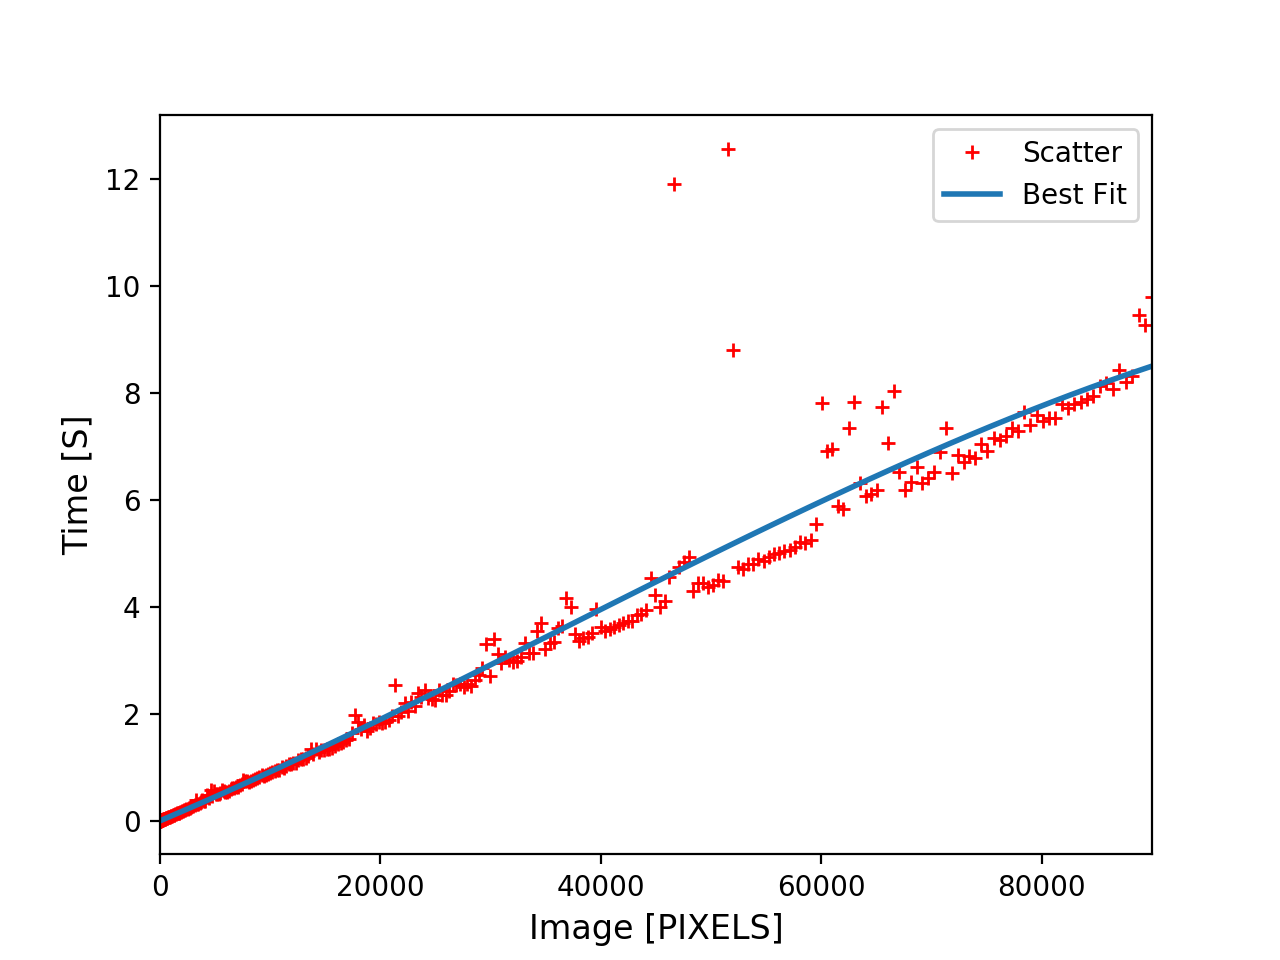
\includegraphics[width=\linewidth]{tests/consecutive.png}
  \caption{Consecutive Testing}
  \label{fig:sub2}
\end{subfigure}
\caption{Scatter Plot  \& Best Fit Curves for Consecutive and Concurrent testing. }
\label{fig:concurrency_test}
\end{figure}


\section{Task Distribution}
\begin{flushleft}
As we have previously worked together, we were more familiar with task distribution. We also decided to both take up on more tasks to share as much of our results and progress as possible. The list below summarizes all of our progress.
\end{flushleft}

\begin{itemize}
    \item Aadil Anil Kumar :
    \begin{itemize}
        \item Wrote the GetPixels/Watershed/DistanceTransform function.
        \item Ran experiments and their respective explanations.
        \item Wrote parts of the report.
        \item Report proof reading.
    \end{itemize}
    \item Otmane Sabir :
    \begin{itemize}
        \item Wrote the getNeighbors/Test script and partially the Watershed function.
        \item Ran one experiment (the nuclei expirement)
        \item Ran the time complexity and the algorithm performance tests.
        \item Wrote parts of the report.
    \end{itemize}
\end{itemize}

\newpage

\begin{thebibliography}{9}
\label{sec:hello}

\bibitem{timecomplexity}
AS Kornillov : \newline
An Overview of Watershed Algorithm Implementations, 
\\\texttt{https://www.mdpi.com/2313-433X/4/10/123/pdf}


\bibitem{parwshed}
Jos B.T.M. Roerdink and Arnold Meijster : \newline
Institute for Mathematics and Computing Science, 
\\\texttt{http://www.cs.rug.nl/roe/publications/parwshed.pdf}


\bibitem{soilletextbook} 
Soille, P. (2010). Morphological image analysis: principles and applications. 
\texttt{Berlin: Springer. Samarin}. 



\end{thebibliography}

\end{document}
